%======================================================================
\section{Introduction}
\label{sec:introduction}
%======================================================================

Learned surrogates of chaotic partial differential equations usually
compress the whole state into one latent vector and learn how that
vector evolves \citep{linotgraham2022,racca2023,ozalpmagri2025}. For
many systems this is the right design. For spatiotemporally chaotic
systems on large domains it is not, for a reason that is structural
rather than technical. Such systems are extensively chaotic: the number
of active degrees of freedom, measured by the Kaplan--Yorke dimension
$\DKY$, grows in proportion to the domain
\citep{ruelle1982,manneville1985,egolfgreenside1994}. A latent vector
fixed at training time has no size to grow into. A model trained on one
domain cannot even be evaluated on another, and every new domain size
requires new data and new training.

We study the alternative: a latent \emph{field}, with a few channels at
each site of a lattice that tiles the physical domain, built only from
operators that are shared by all sites and read a bounded neighbourhood
(Fig.~\ref{fig:concept}).
The parameters of such a model do not depend on the number of sites, so
a model trained at one size is applied to a larger domain by adding
sites, with no retraining. Its latent also has a physical geometry, which
a companion paper uses to build a localized ensemble filter in latent space
\citep{jones2026da}. A local, weight-shared model is
also extensive by construction, like the coupled lattice maps whose
Lyapunov spectra have a thermodynamic limit \citep{livi1986,isola1990}
and can be predicted from small subsystems \citep{carretero1999}. The
question is whether a \emph{learned} local rule reproduces the right
density of chaos, and whether it keeps doing so on domains it was never
trained on.

Two things turn out to matter, and they organize the paper. First, the
data the local rule is learned from. A rule of finite reach can be
learned from a small periodic box, or from windows of one large
simulation, by the same procedure: in both, the sites that border the
scored region are overwritten with data at every step, so the training
loss is that of a limited-area model. Trained on a small box, the rule
transfers in the Kuramoto--Sivashinsky (KS) equation, in
one and in two dimensions. In Kolmogorov flow it transfers only while
the larger domain's large-scale motion stays like the box's; beyond
that, the transferred model drifts into a state with far too much
large-scale energy, and windows of a large simulation are needed.
Second, the propagator must stay chaotic when it runs freely: rollouts
that are too short admit spurious regimes, and longer squared-error
rollouts lower the dimension.

We hold the models to a demanding standard: their own Lyapunov spectra,
computed from the learned maps, compared with spectra of the true PDE at
every domain size, with the uncertainty of the reference measured rather
than assumed. We do this for the one-dimensional KS equation, its two-dimensional
isotropic form, and two-dimensional Kolmogorov flow with linear drag at
three drag coefficients.

\begin{figure*}[htbp]
\centering
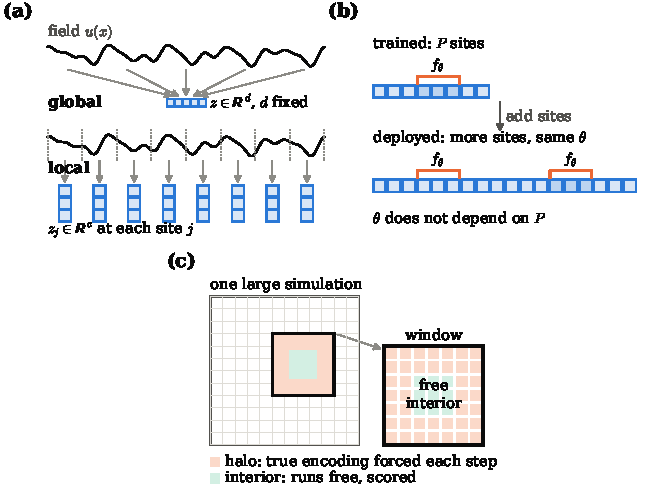
\includegraphics{figures/concept_transfer.pdf}
\caption{The idea in three panels. (a) A global latent compresses the
whole field into one vector of fixed dimension $d$; a local latent field
assigns $c$ channels to the site of each patch. (b) Because every
operator is shared across sites and reads a bounded neighbourhood, the
trained parameters $\theta$ do not depend on the number of sites, and the
model is deployed on a larger domain by adding sites. (c) Training with
a forced halo: at every step of a training rollout the halo of the
window is overwritten by the true encoding, the interior runs free, and
only the interior is scored, so the loss is exactly that of a
limited-area model (Proposition~\ref{prop:halo}). The window can be cut
from one large simulation, as drawn, or be a small periodic box itself
(Sec.~\ref{sec:crop_training}).}
\label{fig:concept}
\end{figure*}

\para{Contributions.}
\begin{itemize}
\item \emph{A local latent field for extensive chaos}
  (Sec.~\ref{sec:method}): weight-shared encoder, decoder and propagator
  of finite reach, equivariant under shifts by whole patches, with a
  parameter count independent of the domain size: $76{,}000$--$135{,}000$
  parameters describe the local law once, and the same parameters run
  domains of any size.
\item \emph{One training procedure, two routes}
  (Sec.~\ref{sec:crop_training}): a forced halo, overwritten with data at
  every step of a training rollout, makes the training loss that of a
  limited-area model, whether the window is a small periodic box or a
  piece of one large simulation.
\item \emph{Zero-shot transfer validated by Lyapunov spectra}
  (Secs.~\ref{sec:results1d} and~\ref{sec:results2d}). Trained at $L=100$,
  a 1D KS model reproduces the true $\DKY$ to within $0.2$--$1.2\%$ from
  $L=50$ to $L=400$, and its whole positive spectrum collapses onto the
  truth's. Trained on a $44^2$ periodic box, three 2D KS models are within
  $3.5\%$ of the truth at $44^2$ and $66^2$, a size never seen in training.
  In 2D the leading exponent is $12$--$30\%$ too high, which we report
  alongside $\DKY$.
\item \emph{Where a small box stops being enough}
  (Sec.~\ref{sec:kolm_box}): in Kolmogorov flow the small-box model fails
  where the truth's large-scale energy grows beyond what the box contains,
  at three times the box width at the strongest drag and at twice it at a
  weaker one. Trained on windows of a simulation sixteen boxes wide, the
  same architecture is within $10\%$ at the two stronger drags.
\item \emph{What fails, and why} (Sec.~\ref{sec:failure}): softmax
  attention, short rollouts and the damping of $\DKY$ by long
  squared-error rollouts, which we connect, as a hypothesis, to the law of
  total variance.
\end{itemize}

What is not new should be said as clearly. Localized reduced models of KS
were built from wavelets a quarter century ago \citep{wittenberg2001},
learned models of KS have reproduced Lyapunov spectra at a single size
\citep{pathak2017,vlachas2020,ozalpmagri2025}, and convolutional
surrogates have been run on larger domains than they were trained on
\citep{barsinai2019,kochkov2021}. Section~\ref{sec:background} places our
results among these. The contrast with minimal flow units, which are
non-extensive by construction and where a global latent vector works
well \citep{constanteamores2025}, is the one-sentence summary of when a
field-valued latent is needed.

Section~\ref{sec:method} defines the model, its structural properties and
the training rule; Section~\ref{sec:systems} describes the three systems
and how precisely their Lyapunov spectra are known.
Sections~\ref{sec:results1d} and~\ref{sec:results2d} report transfer in
one and two dimensions, Section~\ref{sec:failure} the failure modes, and
Section~\ref{sec:discussion} what transfer requires and the limitations
of this study.
